\bookchapter{제42장: 대형 모델 전체 지도와 API 실전}

\chapterintro{앞 장들은 'AI와 어떻게 협업할지'를 다뤘다면, 이번 장은 더 근본적인 질문을 풀어요. '어떤 AI를 쓸까? 어떻게 쓸까?' 2026년 8월 대형 모델 지형은 이미 매우 풍부해요. 국제적으로는 GPT, Claude, Gemini의 3강 경쟁이 벌어지고, 중국에서는 DeepSeek, 퉁이치엔원(Qwen), GLM, Kimi, 더우바오가 만개했죠. 모델마다 저마다의 성격과 특기가 있어요. 잘 고르면 일이 절반의 노력으로 두 배가 되고, 잘못 고르면 두 배의 노력으로 절반만 되죠. 이번 장은 이 모델들을 소개할 뿐 아니라, API로 자기 앱에 연결하는 법과 필요에 맞는 Token Plan(사용량 플랜)을 고르는 법까지 알려 드릴게요.}

\booksection{국제 주류 대형 모델: 3강 구도}

2026년 8월 국제 대형 모델 시장은 OpenAI(GPT 시리즈), Anthropic(Claude 시리즈), Google(Gemini 시리즈)의 3강이 조를 이루는 구도가 되었어요. 각사마다 뚜렷한 특색이 있어요. 하나씩 만나 볼게요.

\booksubsection{OpenAI GPT-5.6 시리즈: 만능 밸런스 올라운더}

OpenAI는 대형 모델 물결의 개척자이고, GPT 시리즈는 지금도 전 세계에서 가장 널리 쓰이는 모델이에요. 2026년 7월에 공개된 GPT-5.6 시리즈는 3단계 포지셔닝 전략을 써요. 플래그십 GPT-5.6 Sol은 고급 추론 수요를 위한 모델이고, 밸런스형 GPT-5.6 Terra는 일상 개발용, 경량형 GPT-5.6 Luna는 높은 동시 처리와 낮은 비용이 필요한 상황용이에요. 세 모델 모두 105만 토큰의 컨텍스트 윈도우를 공유하고 이미지 입력, 함수 호출, 구조화된 출력을 지원해요.

\begin{center}
\begin{tabularx}{\linewidth}{|X|X|X|X|X|}
\hline
\textbf{모델} & \textbf{포지션} & \textbf{입력(/백만 토큰)} & \textbf{출력(/백만 토큰)} & \textbf{컨텍스트 윈도우} \tabularnewline
\hline
GPT-5.6 Sol & 플래그십 추론 & US\$5.00(약 36위안) & US\$30.00(약 217위안) & 105만 토큰 \tabularnewline
GPT-5.6 Terra & 밸런스형 일상 & US\$2.50(약 18위안) & US\$15.00(약 109위안) & 105만 토큰 \tabularnewline
GPT-5.6 Luna & 경량·저비용 & US\$1.00(약 7위안) & US\$6.00(약 44위안) & 105만 토큰 \tabularnewline
\hline
\end{tabularx}
\end{center}

\begin{center}\small\color{gray}OpenAI GPT-5.6 시리즈 가격(2026년 8월)\end{center}

GPT 시리즈의 핵심 강점은 '균형'이에요. 추론, 프로그래밍, 글쓰기, 멀티모달 어디에서도 뚜렷한 약점이 없죠. 여기에 OpenAI의 방대한 플러그인 생태계와 개발자 커뮤니티가 더해져 호환 문서와 도구 체인이 가장 완비되어 있어요. '뭘 골라야 할지 모르겠다'는 상황에서 GPT는 '감으로 골라도 틀리지 않는' 기본 답이에요. 다만 약점도 있어요. 중국 본토에서 접속하려면 특별한 네트워크가 필요하고, 중국어 표현은 이따금 '번역투'가 묻어나며, API 가격은 중상위 수준이에요.

\textbf{좋은 소식}\par

OpenAI는 2026년 8월 무료 사용자의 기본 모델을 GPT-5.6 Luna로 올리고 텍스트 채팅을 무제한으로 열었다고 발표했어요. 즉 비용 없이 GPT의 기본 능력을 체험할 수 있고, 더 강한 추론이나 API 호출이 필요할 때만 결제하면 된다는 뜻이에요.

\booksubsection{Anthropic Claude 시리즈: 프로그래밍과 엄격함의 천장}

GPT가 올라운더라면 Claude는 프로그래밍 분야의 '천장'이에요. Anthropic의 Claude 시리즈는 SWE-bench(소프트웨어 엔지니어링 벤치마크)에서 오랫동안 압도적인 격차로 선두를 달리고, 코드 생성 품질과 엔지니어링급 프로젝트 구현 능력이 업계 1위예요. 더 귀한 점은 Claude의 환각률(거짓 정보를 생성할 확률)이 업계 전체에서 가장 낮은 약 1\% 수준이라는 거예요. 덕분에 학술, 법무 같은 고정밀 상황에 특히 잘 맞아요.

Claude의 또 다른 필살기는 초장문 컨텍스트예요. 100만 토큰의 컨텍스트 윈도우를 지원해 수백 페이지짜리 계약서나 코드베이스 전체를 한 번에 '읽어 내면서' 디테일을 놓치지 않아요. 코드 리팩터링, 긴 문서 분석 같은 상황에서는 사실상 대체가 어려워요. Claude Code는 터미널 AI 프로그래밍 도구로서 2026년 중반까지 연환산 수익 25억 달러를 기록했는데, 이것이 Claude의 프로그래밍 능력이 가장 폭넓게 인정받는 증거예요.

\begin{center}
\begin{tabularx}{\linewidth}{|X|X|X|X|X|}
\hline
\textbf{모델} & \textbf{포지션} & \textbf{입력(/백만 토큰)} & \textbf{출력(/백만 토큰)} & \textbf{컨텍스트 윈도우} \tabularnewline
\hline
Claude Fable 5 & 플래그십 & US\$10.00(약 72위안) & US\$50.00(약 362위안) & 100만 토큰 \tabularnewline
Claude Opus 4.8 & 프로페셔널 & US\$5.00(약 36위안) & US\$25.00(약 181위안) & 100만 토큰 \tabularnewline
Claude Sonnet 5 & 가성비형 & US\$2.00(약 14위안) & US\$10.00(약 72위안) & 100만 토큰 \tabularnewline
\hline
\end{tabularx}
\end{center}

\begin{center}\small\color{gray}Anthropic Claude 시리즈 가격(2026년 8월, Sonnet 5는 할인 가격)\end{center}

Claude의 약점은 가격이에요. Fable 5의 출력 가격은 모든 모델 중 가장 높아 백만 토큰당 50달러에 이르죠. 멀티모달 능력(이미지, 영상 이해)도 상대적으로 약한 편이에요. 예산이 빠듯한 개인 개발자라면 할인 기간의 Sonnet 5 가성비가 매우 돋보여요.

\booksubsection{Google Gemini 시리즈: 멀티모달의 왕}

Google의 Gemini 시리즈는 2026년에 3.1 Pro 버전까지 반복 업그레이드됐어요. Gemini의 최대 필살기는 네이티브 멀티모달이에요. 이미지와 텍스트 분석이 정밀하고, OCR 표 인식이 정확하며, 영상 프레임 추출이 효율적이고 오디오·영상 심층 분석도 지원하죠. Google 생태계(검색, 메일, 클라우드 서비스)와 깊이 묶여 있어 실시간 정보 검색과 모달리티 간 이해에서 두각을 나타내요. Gemini는 200만 토큰의 초장문 컨텍스트 입력도 지원하는, 현재 가장 큰 컨텍스트 윈도우를 가진 모델이에요.

Gemini의 포지션은 '과학 추론과 멀티모달 상황의 첫 선택'이에요. 프로젝트에 이미지 분석, 영상 이해, 과학 계산이 많이 들어간다면 Gemini는 사실상 라이벌이 없어요. 다만 순수 텍스트 코드 생성에서는 Claude보다 조금 뒤처지고, 중국어 표현도 중국제 모델만큼 자연스럽지는 않아요.

\begin{center}
\begin{tabularx}{\linewidth}{|X|X|X|X|}
\hline
\textbf{비교 항목} & \textbf{GPT-5.6} & \textbf{Claude Fable 5} & \textbf{Gemini 3.1 Pro} \tabularnewline
\hline
종합 점수 & 94.8 & 95.0 & 92.1 \tabularnewline
프로그래밍 능력(SWE-bench) & 74.9\% & 64.3\% (Pro) & 보통 \tabularnewline
컨텍스트 윈도우 & 105만 토큰 & 100만 토큰 & 200만 토큰 \tabularnewline
멀티모달 능력 & 균형 잡힘 & 다소 약함 & 가장 강함 \tabularnewline
환각률 & 낮은 편 & 가장 낮음(약 1\%) & 낮은 편 \tabularnewline
중국 내 사용 가능성 & 특수 네트워크 필요 & 특수 네트워크 필요 & 특수 네트워크 필요 \tabularnewline
API 생태계 & 가장 잘 갖춰짐 & 성장 중 & Google 생태계 종속 \tabularnewline
\hline
\end{tabularx}
\end{center}

\begin{center}\small\color{gray}국제 3대 모델 비교(2026년 8월)\end{center}

\begin{tcbwarn}{주의: 중국 내 사용의 현실적인 장벽}
중국 개발자에게 GPT, Claude, Gemini의 가장 큰 걸림돌은 네트워크 접근이에요. Azure 프록시나 API 통합 플랫폼 등을 통해 간접적으로 쓸 수는 있지만, 안정성과 규정 준수 여부는 스스로 판단해야 해요. 프로젝트가 데이터 보안에 엄격한 요구를 한다면 중국산 모델을 우선 고려하는 게 좋아요.

\end{tcbwarn}

\booksection{중국 주요 대형 모델: 다채로운 경쟁}

2026년 중국산 대형 모델은 이미 “추격자”에서 “나란히 달리는 주자”로 변했고, 일부 분야에서는 “선두”까지 달리고 있어요. 2023년의 “껍데기(래퍼)” 논란과 달리, 2026년 중국산 플래그십 모델은 논리 추론, 코드 생성, 중국어 이해 등에서 국제 최상위 모델과 대등하고 격차도 5\% 이내로 줄었어요. 더 중요한 건, 중국산 모델이 중국어 환경·가격·규정에 맞는 배포에서 대체 불가능한 강점을 갖고 있다는 점이에요.

\booksubsection{DeepSeek V4: 가성비의 왕}

DeepSeek(딥시크)는 중국산 대형 모델 가운데 현상급 존재예요. 2025년 초 DeepSeek-V3는 “GPT보다 10분의 1 가격인데 성능은 맞먹는다”는 포지셔닝으로 시장을 뒤흔들었고, 업계에서는 “범용 AI 대형 모델의 킬러 라인”이라 불렀어요. — 이보다 저렴한 모델은 성능이 뒤지고, 이보다 비싼 모델은 가성비에서 앞서지 못한다는 뜻이죠. 2026년 8월에는 DeepSeek V4-Pro 정식 버전이 출시됐어요: 1.6조 파라미터 MoE 아키텍처, 활성 파라미터 약 49B, 100만 토큰 무손실 컨텍스트 지원, 코드 가성비는 세계 최고봉으로 평가받아요.

DeepSeek V4는 에이전트 능력에서 큰 도약을 이뤘어요. — DeepSWE 벤치마크는 12.8에서 62.7(+390\%)로, NL2Repo는 38.5에서 61.5로 올랐습니다. API에는 Responses API와 Anthropic API 이중 프로토콜 지원이 새로 추가되어 Codex, Claude Code 같은 주요 코딩 도구와 호환돼요. 즉 Claude API 대신 DeepSeek API를 Claude Code에서 쓸 수 있다는 뜻이에요. — 비용은 몇 배로 줄고 사용 경험은 거의 같아요.

\begin{center}
\begin{tabularx}{\linewidth}{|X|X|X|X|X|}
\hline
\textbf{모델명} & \textbf{포지셔닝} & \textbf{입력(/100만 토큰)} & \textbf{출력(/100만 토큰)} & \textbf{컨텍스트 윈도우} \tabularnewline
\hline
DeepSeek V4 Pro & 플래그십 추론 & 3위안 (약 US\$0.43) & 6위안 (약 US\$0.87) & 100만 토큰 \tabularnewline
DeepSeek V4 Flash & 경량·고속 & 1위안 (약 US\$0.14) & 2위안 (약 US\$0.28) & 100만 토큰 \tabularnewline
\hline
\end{tabularx}
\end{center}

\begin{center}\small\color{gray}DeepSeek V4 시리즈 가격표(2026년 8월, 프로모션 가격)\end{center}

가격 비교: 입력 100만 토큰 + 출력 100만 토큰 기준으로 DeepSeek V4 Flash는 약 0.42달러, GPT-5.6 Sol은 약 35달러, Claude Fable 5는 약 60달러가 들어요. 격차가 최대 80\textasciitilde{}140배에 달하죠.

\textbf{주의: DeepSeek 가격 인상 예정}\par

DeepSeek 공식 측은 2026년 8월 6일 “조만간 API 가격을 크게 인상할 계획”이라고 공지했어요. 프로모션 가격은 오래 지속되지 않을 수 있습니다. 일부 언론은 인상폭이 30배에 이를 수 있다고 전하지만, 8월 14일 기준 아직 최종 조정안은 발표되지 않았어요. 게다가 DeepSeek V4 정식 버전에는 시간대별(피크·비피크) 가격제가 도입되어 피크 시간대 호출 비용은 두 배가 됩니다. 최신 가격은 공식 공지를 확인해 보세요.

\booksubsection{퉁이치엔원 Qwen3.7 Max: 알리바바 클라우드의 기업용 선택}

알리바바 클라우드의 퉁이치엔원(Qwen) 시리즈는 알리바바 클라우드 생태계를 바탕으로 기업용 배포에서 타고난 강점을 지녀요. 2026년 7월의 Qwen3.7 Max가 현재의 플래그십입니다: 235B 파라미터 밀집(dense) 모델, 256K 네이티브 컨텍스트, 최대 1M까지 확장 가능. Qwen의 핵심 강점은 성숙한 오픈소스 생태계(7B부터 235B까지 전 시리즈 오픈소스), 정확한 중국어 상황 이해, 알리바바 클라우드 인프라와의 깊은 통합이에요.

\begin{center}
\begin{tabularx}{\linewidth}{|X|X|X|}
\hline
\textbf{모델명} & \textbf{출력 가격(/100만 토큰)} & \textbf{적합한 용도} \tabularnewline
\hline
qwen-turbo & 0.6위안 & 간단한 질의응답, 텍스트 분류, 대량 동시 처리 \tabularnewline
qwen-long & 2.0위안 & 10M 초장문 컨텍스트 처리 \tabularnewline
qwen3.7-flash & 7.2위안 & 범용 대화, 콘텐츠 생성 \tabularnewline
qwen3.7-plus & 12.0위안 & 멀티모달(이미지+영상), 중국어 창작 \tabularnewline
qwen3.7-max & 36.0위안 & 최상위 중국어 능력, 복잡한 작업 \tabularnewline
\hline
\end{tabularx}
\end{center}

\begin{center}\small\color{gray}퉁이치엔원 Qwen 시리즈 단계별 가격(2026년 8월)\end{center}

Qwen 가격은 단계별 전략을 써요. — 초저가의 qwen-turbo(출력 0.6위안/100만 토큰)부터 플래그십 qwen3.7-max(출력 36위안/100만 토큰)까지, 가벼운 질의응답부터 복잡한 추론까지 모든 상황의 수요를 커버하죠. 이미 알리바바 클라우드를 쓰는 기업에게 Qwen은 가장 손쉬운 통합 선택이에요.

\booksubsection{즈푸 GLM-5.1: 중국산 SWE-bench 1위}

즈푸 AI의 GLM 시리즈는 2026년에 돋보이는 성과를 냈어요. GLM-5.1은 SWE-bench에서 중국산 모델 중 1위를 차지했습니다: 744B MoE 밀집 하이브리드 아키텍처, 100만 컨텍스트 지원. 특징은 정확한 중국어 의미 이해와 중국 내 규정에 맞는 온프레미스 배포 지원이에요. — 데이터 보안 요구가 높은 금융·공공 분야에서 아주 중요한 부분이죠. GLM-5.1 가격은 100만 토큰당 입력 6위안, 출력 24위안으로 중국산 모델 중 중간 수준이에요.

\booksubsection{Kimi K3: 초장문 텍스트의 왕}

문샷 AI(Moonshot AI)의 Kimi 시리즈는 초장문 텍스트 처리 능력으로 유명해요. 2026년 7월에 나온 Kimi K3는 2.8조 파라미터 규모를 자랑하며 여러 복잡 작업 평가에서 세계 최상위권에 들었어요. Kimi의 핵심 상황은 긴 코드베이스 분석과 긴 문서 검색 증강(RAG)입니다. — 책 한 권 분량의 텍스트나 프로젝트 전체 코드도 처리할 수 있고, “바다에서 바늘 찾기”식 검색 작업에서 뛰어난 성능을 보이죠. Kimi 가격은 상대적으로 높은 편(출력 약 12\textasciitilde{}20위안/100만 토큰)이지만, 장문 상황에서의 가성비는 따라올 수 없어요.

\booksubsection{더우바오(Doubao): 바이트댄스의 만능 선수}

바이트댄스의 더우바오 시리즈는 2026년에도 꾸준한 모습을 보였어요. Doubao Seed 2.1 Pro는 화산엔진의 플래그십 모델로, 256K 컨텍스트에 실측에서도 전반적으로 안정적인 성능을 보이고 중국어 상황 체험이 특히 돋보여요. 더우바오의 강점은 가입하면 대량의 무료 토큰을 바로 준다는 것, 화산엔진 생태계 통합이 잘 갖춰져 있다는 것, 그리고 가격이 중국 최저가 권역에 속한다는 것이에요. AI 코딩을 빨리 체험해 보고 싶은 초보자에게 더우바오는 진입 장벽이 없는 입문 선택이에요.

\begin{center}
\begin{tabularx}{\linewidth}{|X|X|X|X|X|X|}
\hline
\textbf{비교 항목} & \textbf{DeepSeek V4} & \textbf{Qwen3.7 Max} & \textbf{GLM-5.1} & \textbf{Kimi K3} & \textbf{더우바오 2.1 Pro} \tabularnewline
\hline
종합 점수 & 87.5 & 89.7 & 90.5 & 88+ & 85+ \tabularnewline
코딩 능력 & 매우 강함 & 강함 & 중국산 SWE 1위 & 강함 & 중상위 \tabularnewline
중국어 이해 & 우수함 & 우수함 & 정확함 & 우수함 & 우수함 \tabularnewline
컨텍스트 윈도우 & 100만 & 256K-1M & 100만 & 초장문 & 256K \tabularnewline
출력 가격(위안/M) & 6 & 36 & 24 & 12-20 & 30 \tabularnewline
오픈소스 & MIT 라이선스 & 전 시리즈 오픈소스 & 부분 오픈소스 & 비공개 & 비공개 \tabularnewline
온프레미스 배포 & 지원 & 지원 & 지원 & 미지원 & 미지원 \tabularnewline
\hline
\end{tabularx}
\end{center}

\begin{center}\small\color{gray}중국 5대 모델 비교(2026년 8월)\end{center}

주목할 중요한 추세 하나: 중국산 모델과 GPT/Claude 사이의 “세대차” 느낌은 사라졌어요. 논리 추론과 수학 경진에서는 중국산 플래그십과 GPT-5의 점수 차이가 거의 한 자릿수입니다. 체계적인 아키텍처 사고와 복잡한 엔지니어링 추론에서는 Claude가 여전히 앞서요. — 더 “영감”이 있는 아키텍처 안을 내놓는 반면 중국산 모델은 때때로 “교과서적”으로 보이거든요. 하지만 중국어 상황, 비용 통제, 규정에 맞는 배포에서는 중국산 모델이 압도적인 우위예요.

\begin{center}
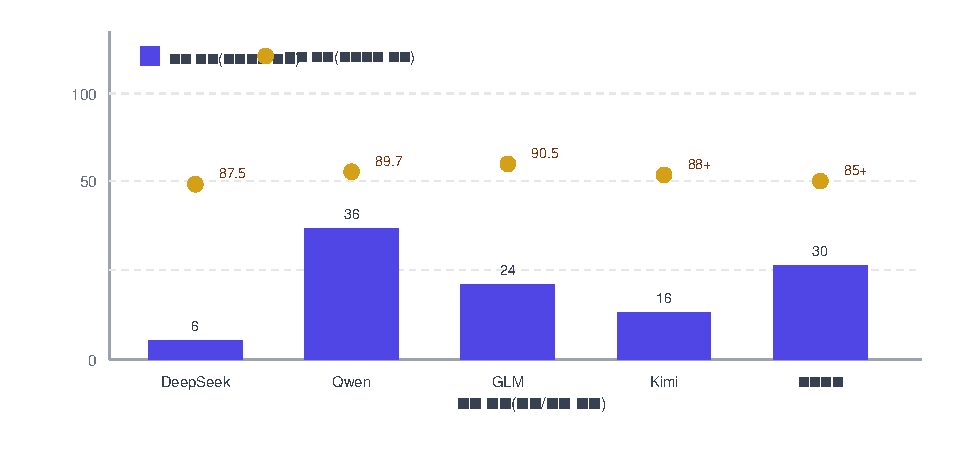
\includegraphics[width=0.92\linewidth]{figures/fig-di-si-shi-er-zhang-1}
\\[2pt]\small 그림 4: 5개 모델 가격·성능 비교(가격은 낮을수록, 점수는 높을수록 좋음)
\end{center}

\booksection{모델 선택 의사결정 프레임워크}

각 모델의 특징을 알았으니, 내 프로젝트에는 어떤 모델이 맞을까요? “네 가지 질문 의사결정법”을 드릴게요. — 네 가지 질문에 답하기만 하면 가장 잘 맞는 모델을 좁힐 수 있어요.

프로젝트 배포는 중국인가요, 해외인가요?

중국 국산 모델 선택

|

해외 해외 모델도 선택 가능

핵심 작업은 코딩인가요, 다른 것인가요?

코딩 Claude 또는 DeepSeek

|

기타 계속 판단

초장문맥(>50만 토큰)이 필요한가요?

필요 Gemini 또는 Kimi

|

불필요 계속 판단

예산에 민감한가요?

민감 DeepSeek 또는 Qwen-turbo

|

아니요 GPT-5.6 또는 Claude

\begin{center}\small\color{gray}그림 5: 대형 모델 선택 네 가지 질문 의사결정법\end{center}

\begin{tcbinfo}{꿀팁: 조합 전략}
이 의사결정법이 교리는 아니에요. — 많은 상황에서 여러 모델을 조합해 써야 하거든요. 흔한 조합 전략 하나: 일상 개발에는 DeepSeek이나 Qwen(비용 저렴, 중국어 강점), 핵심 아키텍처 설계에는 Claude(추론 강함, 환각 적음), 멀티모달 분석에는 Gemini(이미지·영상 처리). “모델 하나로 끝까지 가는” 게 아니라 필요에 따라 모델을 갈아타세요.

\end{tcbinfo}

\booksection{API 호출 입문: 제로부터 대형 모델 연동하기}

많은 AI 코딩 강좌는 대화 화면 쓰는 법만 가르치지만, 진짜 “AI 코딩” — 내 앱이 대형 모델을 호출하게 만드는 것 — 은 API를 통해야 해요. API(Application Programming Interface, 애플리케이션 프로그래밍 인터페이스)는 프로그램 사이의 통신 규약이에요. API를 통해 내 코드는 함수를 호출하듯 대형 모델의 능력을 호출할 수 있어요.

\booksubsection{토큰(Token)이란?}

API를 알기 전에 먼저 “토큰(Token)” 개념을 이해해야 해요. 토큰은 대형 모델 과금의 기본 단위로, “AI의 읽기·쓰기 단위”라고 이해하면 돼요. 토큰 하나는 대략 영어 0.75 단어(4문자), 중국어 0.5\textasciitilde{}1자에 해당해요. 1000자 분량의 중국어 텍스트는 약 1500\textasciitilde{}2000개의 토큰을 소모해요.

토큰은 글자 수도 문자 수도 아니에요. 대형 모델은 전용 토크나이저(Tokenizer)로 텍스트를 토큰으로 쪼개죠. 같은 단어라도 모델에 따라 토큰 수가 달라질 수 있어요. — 예컨대 “인공지능”이라는 단어는 GPT에서는 3개, DeepSeek에서는 2개일 수 있어요. 대부분 모델의 API는 실제 소모된 토큰 수를 돌려주므로 API 응답에서 확인할 수 있어요.

\begin{tcbinfo}{토큰 비용 빠르게 계산하기}
중국어 100만 자는 약 150만 토큰에 해당해요. DeepSeek V4 Flash로 입력 100만 자 + 출력 100만 자를 처리하면 약 0.42달러(약 3위안), Claude Fable 5로 같은 양을 처리하면 약 60달러(약 434위안)가 들어요. 모델 선택이 프로젝트 비용에 직결되는 이유죠.

\end{tcbinfo}

\booksubsection{API 키 발급받기}

대형 모델 API를 쓰는 첫걸음은 API 키 발급이에요. — 신원 인증에 쓰이는 열쇠 문자열이죠. 모델 제공사마다 자체 API 플랫폼이 있으니, 계정에 가입하고 API 키를 만들어야 해요. 주요 모델의 API 플랫폼 입구와 발급 절차는 다음과 같아요:

\begin{center}
\begin{tabularx}{\linewidth}{|X|X|X|X|}
\hline
\textbf{모델} & \textbf{API 플랫폼} & \textbf{발급 절차} & \textbf{무료 크레딧} \tabularnewline
\hline
DeepSeek & platform.deepseek.com & 가입 실명 인증 API 키 생성 & 신규 사용자 증정 크레딧 \tabularnewline
퉁이치엔원 & bailian.aliyun.com(바이롄 플랫폼) & 알리바바 클라우드 계정 로그인 서비스 개통 키 생성 & 신규 사용자 무료 체험 \tabularnewline
즈푸 GLM & open.bigmodel.cn & 가입 실명 인증 API 키 생성 & 신규 사용자 증정 크레딧 \tabularnewline
Kimi & platform.moonshot.cn & 가입 실명 인증 API 키 생성 & 제한적 무료 크레딧 \tabularnewline
더우바오 & volcengine.com(화산엔진) & 가입 Ark 서비스 개통 API 키 생성 & 가입 시 대량 토큰 증정 \tabularnewline
OpenAI GPT & platform.openai.com & 가입 신용카드 등록 API 키 생성 & 무료 크레딧 없음(유료 필요) \tabularnewline
Anthropic Claude & console.anthropic.com & 가입 카드 등록 API 키 생성 & 신규 사용자 소량 크레딧 \tabularnewline
\hline
\end{tabularx}
\end{center}

\begin{center}\small\color{gray}주요 모델 API 플랫폼 및 키 발급 방법(2026년 8월)\end{center}

\textbf{보안 주의: API 키 = 지갑 비밀번호}\par

API 키는 지갑 비밀번호와 같아요. — 키를 손에 넣은 사람은 누구나 내 크레딧으로 모델을 호출할 수 있거든요. 그러니: API 키를 코드에 적지 마세요(환경 변수로 관리). 키가 든 코드를 공개 Git 저장소에 커밋하지 마세요. 키가 보이는 스크린샷을 소셜 미디어에 올리지도 마세요. 키가 유출됐다면 즉시 플랫폼에서 삭제하고 다시 만드세요.

\booksubsection{첫 번째 API 호출}

API 키를 받았다면 어떤 프로그래밍 언어로도 대형 모델 API를 호출할 수 있어요. 아래는 Python으로 가장 단순한 호출을 보여주는 예시예요. — DeepSeek에 메시지 한 개를 보내고 답장을 받아요.

\begin{lstlisting}[language=Python]
# SDK 설치: pip install openai
# DeepSeek는 OpenAI SDK 형식과 호환되므로 바로 쓸 수 있어요
from openai import OpenAI
import os

# 1. 클라이언트 생성(API 키는 환경 변수에서 읽음)
client = OpenAI(
    api_key=os.environ.get("DEEPSEEK_API_KEY"),
    base_url="https://api.deepseek.com"
)

# 2. 요청 전송
response = client.chat.completions.create(
    model="deepseek-chat",  # 모델 지정
    messages=[
        {"role": "system", "content": "당신은 파이썬 코딩 어시스턴트예요."},
        {"role": "user", "content": "퀵 정렬 함수를 작성해 주세요."}
    ]
)

# 3. 응답 받기
print(response.choices[0].message.content)

# 4. 토큰 소비 확인
print(f"입력 토큰: {response.usage.prompt_tokens}")
print(f"출력 토큰: {response.usage.completion_tokens}")
print(f"총 토큰: {response.usage.total_tokens}")
\end{lstlisting}

이 코드의 핵심 로직은: 클라이언트 생성(API 키와 모델 주소를 담아) 메시지 목록 구성(system은 역할 설정, user는 사용자 입력) 요청 전송 답변 수신이에요. 이 패턴은 OpenAI 형식과 호환되는 거의 모든 모델에 적용돼요. — api\_key와 base\_url만 바꾸면 모델을 갈아탈 수 있죠. 많은 중국산 모델이 OpenAI SDK 형식 호환을 택하는 이유이기도 해요: 개발자는 코드 두 줄만 고치면 모델을 바꿀 수 있어 전환 비용이 극히 낮아요.

다음은 다른 모델로 바꿀 때의 코드 차이예요. — 딱 두 줄만 고치면 된다는 점에 주목하세요:

\begin{lstlisting}[language=Python]
# DeepSeek
client = OpenAI(
    api_key=os.environ.get("DEEPSEEK_API_KEY"),
    base_url="https://api.deepseek.com"
)
# model="deepseek-chat"

# 퉁이치엔원(바이롄 플랫폼)
client = OpenAI(
    api_key=os.environ.get("DASHSCOPE_API_KEY"),
    base_url="https://dashscope.aliyuncs.com/compatible-mode/v1"
)
# model="qwen-plus"

# 지푸 GLM
client = OpenAI(
    api_key=os.environ.get("GLM_API_KEY"),
    base_url="https://open.bigmodel.cn/api/paas/v4"
)
# model="glm-4"

# OpenAI GPT
client = OpenAI(
    api_key=os.environ.get("OPENAI_API_KEY"),
    # base_url은 기본값 그대로 쓰면 돼요
)
# model="gpt-5.6-terra"
\end{lstlisting}

\booksubsection{스트리밍 응답 처리}

실제 앱에서는 AI가 전부 쓸 때까지 기다렸다가 한꺼번에 보여주길 원하지 않을 거예요. — 사용자가 너무 오래 기다리게 되거든요. 스트리밍 응답(Streaming)을 쓰면 AI가 생성하는 동시에 한 글자씩 보여줄 수 있어 사용자 경험이 크게 좋아져요. 타자기처럼 글자가 하나하나 튀어나오는 모습이라 사용자가 느끼는 차이는 완전히 달라요.

\begin{lstlisting}[language=Python]
# 스트리밍 응답: 한 글자씩 출력
stream = client.chat.completions.create(
    model="deepseek-chat",
    messages=[
        {"role": "user", "content": "파이썬 버블 정렬 튜토리얼을 작성해 주세요"}
    ],
    stream=True  # 스트리밍 응답 켜기
)

# 청크 단위로 받아 출력
for chunk in stream:
    if chunk.choices[0].delta.content is not None:
        print(chunk.choices[0].delta.content, end="", flush=True)
# 출력이 타이핑 기계처럼 한 글자씩 표시돼요
\end{lstlisting}

\booksection{토큰 플랜(Token Plan) 구매 가이드}

대부분의 모델 제공사는 두 가지 과금 방식이 있어요: 종량제(Pay-as-you-go)와 플랜 구독(Token Plan / Subscription). 두 방식의 차이를 이해하면 사용 비용을 크게 줄일 수 있어요.

\booksubsection{종량제 vs 플랜 구독}

\begin{center}
\begin{tabularx}{\linewidth}{|X|X|X|}
\hline
\textbf{구분} & \textbf{종량제(Pay-as-you-go)} & \textbf{플랜 구독(Subscription)} \tabularnewline
\hline
과금 방식 & 쓴 토큰만큼 결제 & 고정 요금 선결제 후 크레딧 사용 \tabularnewline
적합한 상황 & 사용량 불안정, 가끔 호출 & 사용량 안정, 고빈도 호출 \tabularnewline
가격 이점 & 표준 가격 & 종량제보다 20\textasciitilde{}50\% 저렴 \tabularnewline
유연성 & 언제든 사용 가능, 약정 없음 & 선결제 필요, 크레딧 만료 시 소멸될 수 있음 \tabularnewline
초과분 처리 & 자동 종량 과금 & 크레딧 초과 시 종량제로 전환 \tabularnewline
대표 플랫폼 & 각 모델 공식 API 플랫폼 & OpenAI Plus/Pro, Claude Pro, Cursor Pro \tabularnewline
\hline
\end{tabularx}
\end{center}

\begin{center}\small\color{gray}두 가지 과금 방식 비교\end{center}

초보자라면 종량제부터 시작하는 걸 권해요. — 선결제 없이 쓴 만큼만 내면 되니까요. 월 사용량이 일정 수준(예: 매달 50위안 이상)으로 안정되면, 그때 더 낮은 단가를 위해 플랜 구독으로 바꾸는 걸 고려해 보세요.

\booksubsection{주요 구독 플랜 한눈에 보기}

\begin{center}
\begin{tabularx}{\linewidth}{|X|X|X|X|}
\hline
\textbf{플랜} & \textbf{월 요금} & \textbf{포함 내용} & \textbf{추천 대상} \tabularnewline
\hline
ChatGPT Free & 무료 & GPT-5.6 Luna 무제한 텍스트 대화 & 입문자 체험용 \tabularnewline
ChatGPT Plus & US\$20/월 & GPT-5.6 Sol, 이미지 생성, 데이터 분석, 플러그인 이용 & 중간 수준 사용자 \tabularnewline
ChatGPT Pro & US\$200/월 & 모든 모델 무제한 사용, 신기능 우선 접근 & 고강도 전문 사용자 \tabularnewline
Claude Free & 무료 & 횟수 제한 Claude 대화 & 입문자 체험용 \tabularnewline
Claude Pro & US\$20/월 & Claude 무제한 사용, 신모델 우선 접근 & 코딩 개발자 \tabularnewline
Cursor Free & 무료 & 횟수 제한 AI 자동완성·대화 & 초보자 체험용 \tabularnewline
Cursor Pro & US\$20/월 & 무제한 AI 자동완성, 월 500회 프리미엄 요청 & 일상 개발자 \tabularnewline
Cursor Business & US\$40/월/인 & 팀 협업, 관리 콘솔, 프라이버시 모드 & 팀 사용 \tabularnewline
\hline
\end{tabularx}
\end{center}

\begin{center}\small\color{gray}주요 AI 도구 구독 플랜(2026년 8월)\end{center}

중국 모델들의 구독 방식은 조금 달라요. DeepSeek는 주로 종량제라 월 구독 플랜이 없어요. — 충전한 뒤 실제 사용량만큼 차감돼요. 퉁이치엔원은 바이롄 플랫폼에서 선불 리소스 패키지(일정량의 토큰 크레딧을 할인가에 구매)를 제공하고, 더우바오도 화산엔진에서 비슷한 선불 방식을 제공해요. 중국 개발자에게 가장 경제적인 조합은 보통 DeepSeek 종량제(일상 개발) + 더우바오 무료 크레딧(체험·테스트)이에요.

\booksubsection{API 통합 플랫폼}

여러 모델을 동시에 써야 한다면 API 통합(어그리게이션) 플랫폼이 편리한 선택이에요. 통합 플랫폼은 API 키 하나만으로 전 세계 수십 종 모델을 호출할 수 있게 해 줘서, 플랫폼마다 따로 가입할 필요가 없어요.

\begin{center}
\begin{tabularx}{\linewidth}{|X|X|X|X|}
\hline
\textbf{플랫폼} & \textbf{특징} & \textbf{가격 이점} & \textbf{적합한 상황} \tabularnewline
\hline
OpenRouter (openrouter.ai) & 해외 통합 플랫폼, 키 하나로 글로벌 모델 호출 & 가격 투명, 실시간 가격 비교 지원 & 여러 해외 모델을 유연하게 전환할 때 \tabularnewline
SiliconFlow (siliconflow.cn) & 중국 통합 플랫폼, 다양한 중국산 모델 API 제공 & 공식 가격보다 20\textasciitilde{}30\% 저렴 & 중국 개발자, 여러 모델 가격 비교 \tabularnewline
Azure OpenAI (마이크로소프트 제공) & 마이크로소프트 Azure를 통해 제공되는 OpenAI API & Batch API 50\% 할인 & 엔터프라이즈 OpenAI 호출, 대량 비동기 작업 \tabularnewline
바이두 첸판(qianfan.baidubce.com) & 바이두 AI 클라우드 플랫폼, ERNIE 등 모델 제공 & 신규 사용자 증정 크레딧 & 바이두 생태계 사용자 \tabularnewline
\hline
\end{tabularx}
\end{center}

\begin{center}\small\color{gray}주요 API 통합 플랫폼(2026년 8월)\end{center}

\textbf{주의: “공유 키” 구매 금지}\par

타오바오, 셴위 같은 플랫폼에서 이른바 “공유 API 키”를 사지 마세요. — 이런 키는 출처가 불분명해 언제든 계정이 정지될 수 있고, 데이터 유출 위험도 있어요. API 키는 반드시 공식 플랫폼이나 정식 통합 플랫폼을 통해 받으세요.

\booksubsection{비용 최적화 전략}

모델을 잘 고르는 건 첫걸음일 뿐, “아끼면서 쓰는 법”도 똑같이 중요해요. 다음은 실전에서 검증된 비용 최적화 전략 몇 가지예요:

\begin{enumerate}
  \item 캐시 히트를 잘 활용하세요. 많은 모델이 “캐시” 기능을 제공해요. — 요청에 이전에 처리했던 내용(예: 시스템 프롬프트)이 포함되면 그 부분은 아주 낮은 가격으로만 과금되죠. DeepSeek의 캐시 히트 가격은 일반 가격의 1/60에 불과해요. 고정된 시스템 프롬프트를 메시지 목록 맨 앞에 두면 캐시 히트를 극대화할 수 있어요.
  \item 단계별 라우팅 — 간단한 작업은 저렴한 모델로, 복잡한 작업은 비싼 모델로 처리하세요. 예컨대 텍스트 분류는 DeepSeek V4 Flash(출력 2위안/100만 토큰), 아키텍처 설계는 Claude(출력 181위안/100만 토큰)로요. 프로젝트 호출의 80\%는 저렴한 모델로 처리할 수 있어요.
  \item 출력 길이 제한. API는 출력 토큰 기준으로 과금되므로 출력이 길수록 비싸져요. 장문이 필요 없는 상황에서는 max\_tokens 파라미터로 출력 길이를 제한해 AI가 “불필요하게 장황해지는” 걸 막으세요.
  \item 실시간이 아닌 작업은 Batch API로 처리. 즉시 응답이 필요 없는 작업이 대량으로 있다면(예: 대량 데이터 라벨링, 문서 요약) Batch API로 50\% 할인을 받을 수 있어요. OpenAI와 Azure 모두 이 기능을 제공해요.
  \item 토큰 사용량 모니터링. 대부분의 API 플랫폼은 사용량 통계 패널을 제공해요. 주기적으로 사용량 분포를 살펴 토큰을 가장 많이 쓰는 호출을 찾아 맞춤으로 최적화하세요. 사소한 프롬프트 조정 하나(예: “자세히 설명해 주세요”를 “세 문장으로 설명해 주세요”로 바꾸기)로도 토큰을 50\% 아낄 수 있어요.
\end{enumerate}

\begin{center}
\begin{tabularx}{\linewidth}{|X|X|X|X|}
\hline
\textbf{최적화 전략} & \textbf{절감 폭} & \textbf{실행 난이도} & \textbf{설명} \tabularnewline
\hline
캐시 히트 & 최대 98\% & 낮음 & 고정 내용을 메시지 앞부분에 배치 \tabularnewline
단계별 라우팅 & 50\%-80\% & 중간 & 간단한 작업은 저렴한 모델 사용 \tabularnewline
출력 길이 제한 & 30\%-60\% & 낮음 & max\_tokens 파라미터 설정 \tabularnewline
Batch API & 50\% & 낮음 & 비실시간 작업은 배치 처리 \tabularnewline
프롬프트 최적화 & 20\%-50\% & 중간 & 프롬프트 간결화, 군더더기 줄이기 \tabularnewline
\hline
\end{tabularx}
\end{center}

\begin{center}\small\color{gray}비용 최적화 전략과 효과(2026년 8월)\end{center}

\booksection{실전: 프로젝트에 대형 모델 API 연동하기}

이번 장을 하나의 완성된 실전으로 마무리해 봐요. — “AI 요약 생성기”를 만드는 거예요: 사용자가 긴 텍스트를 입력하면 대형 모델 API를 호출해 요약을 생성해요. 이 실전은 API 호출의 전체 흐름을 보여줘요: 환경 설정, API 호출, 오류 처리, 비용 통제.

\begin{lstlisting}[language=Python]
# ai_summarizer.py - AI 요약 생성기
import os
from openai import OpenAI

# 1. 설정(API 키는 환경 변수에서 읽어요, 절대 하드코딩 금지)
client = OpenAI(
    api_key=os.environ.get("DEEPSEEK_API_KEY"),
    base_url="https://api.deepseek.com"
)

def summarize(text: str, max_length: int = 200) -> dict:
    """텍스트 요약 생성

    Args:
        text: 요약할 원문
        max_length: 요약 최대 길이(토큰 수)

    Returns:
        dict: 요약과 토큰 소비 정보 포함
    """
    try:
        response = client.chat.completions.create(
            model="deepseek-chat",
            messages=[
                {
                    "role": "system",
                    "content": "당신은 요약 생성기예요."
                               "사용자가 제공한 텍스트를 간결하게 요약하세요."
                               "요약은 3문장을 넘지 않게 하세요."
                },
                {
                    "role": "user",
                    "content": f"다음 텍스트를 요약해 주세요:\n\n{text}"
                }
            ],
            max_tokens=max_length,  # 출력 길이 제한
            temperature=0.3  # 낮은 온도=더 안정적
        )

        return {
            "success": True,
            "summary": response.choices[0].message.content,
            "input_tokens": response.usage.prompt_tokens,
            "output_tokens": response.usage.completion_tokens,
            "total_tokens": response.usage.total_tokens
        }

    except Exception as e:
        return {
            "success": False,
            "error": str(e)
        }

# 2. 사용 예시
if __name__ == "__main__":
    long_text = """
    (긴 텍스트를 붙여넣으세요...)
    """

    result = summarize(long_text)

    if result["success"]:
        print(f"요약: {result['summary']}")
        print(f"소비 토큰: {result['total_tokens']}")
        # 비용 추정: DeepSeek V4 Flash
        cost = result['total_tokens'] * 0.000004  # 약 0.4펀/천 토큰
        print(f"예상 비용: {cost:.4f}위안")
    else:
        print(f"오류 발생: {result['error']}")
\end{lstlisting}

이 코드에는 API 호출의 모범 사례 몇 가지가 담겨 있어요: API 키는 환경 변수로 읽어 코드에 절대 하드코딩하지 않기, 함수에 명확한 문서와 타입 힌트 두기, max\_tokens로 출력 길이 제한하기, temperature를 낮은 값(0.3)으로 두어 더 안정적인 출력 얻기, 완전한 오류 처리 갖추기, 비용 추적을 위해 토큰 소모 정보 돌려주기. AI에게 이 코드를 시킬 때는 이 요구사항들을 그대로 말해 주세요. — AI는 충분히 구현해 줄 수 있어요.

이 장의 마지막 교훈: 모델은 "탄약"이고 방법론은 "전술"이에요. 알맞은 탄약을 고르면 싸움이 수월해지지만, 좋은 전술이 없으면 아무리 좋은 탄약도 전쟁을 이길 수 없어요. 각 모델의 특성과 API 사용법을 알았으니 이제 넉넉한 "탄약고"가 생긴 셈이에요 — 하지만 이 전투를 어떻게 치를지는 앞 장에서 배운 사고 방법론에 달렸어요.

\begin{tcbpractice}{직접 해보기: 첫 API 호출 성공하기}
중국산 모델 플랫폼 하나에 가입하고(DeepSeek이나 즈푸 추천, 둘 다 신규 사용자 크레딧을 줘요), API 키를 만들어 시스템 환경 변수에 넣은 뒤(코드가 아니에요!), 위의 “첫 번째 API 호출” 코드를 실행해 보세요. AI의 답장이 출력되는 순간, 여러분은 “AI를 쓰는 사람”과 “AI 앱을 만드는 사람” 사이의 경계선을 넘은 거예요.

\end{tcbpractice}

\begin{tcbsummary}{이번 장 정리}
\begin{itemize}
  \item 국제 3강: GPT-5.6(균형 잡힌 만능), Claude(코딩 최강 + 환각률 1\%), Gemini(멀티모달의 왕 + 200만 컨텍스트)
  \item 중국 5강: DeepSeek V4(가성비의 왕, 가격 인상 공지 주의), Qwen3.7(엔터프라이즈), GLM-5.1(SWE 중국산 1위), Kimi K3(초장문), 더우바오(무료 입문)
  \item 네 가지 질문 의사결정법: 배포 위치는? 코딩인가 다른 용도인가? 초장문 컨텍스트가 필요한가? 예산에 민감한가?
  \item 토큰은 과금 단위: 중국어 1자당 약 1.5\textasciitilde{}2 토큰, 100만 자는 약 150만 토큰
  \item API 키 = 지갑 비밀번호: 환경 변수로 관리, 하드코딩 절대 금지, Git 업로드 금지
  \item 중국산 모델은 대부분 OpenAI SDK와 호환: 모델 교체는 api\_key와 base\_url 두 줄만 바꾸면 끝
  \item 비용 절약 5가지: 캐시 히트, 단계별 라우팅, 출력 제한, Batch API, 사용량 모니터링
\end{itemize}

\end{tcbsummary}
